\chapter{Data and simulated samples}\label{chap:datamc}

\section{Data}
The analysis presented in this thesis is performed on \emph{\protonproton} collision data collected by ATLAS and delivered by the LHC Run-2, between 2015 and 2018, corresponding to a total integrated luminosity of \SI{139}{\femto\barn^{-1}}. The breakdown of the luminosity collected in each year by ATLAS available for physics analysis is outlined in \cref{tab:data:lumi}. The luminosity uncertainty is determined from calibration of the luminosity scale using the Van Der Meer scans described in \cref{sec:lumi}. 
\begin{table}[h]
    \centering
    \begin{tabular}{l|c}
        Year & luminosity [\SI{}{\femto\barn^{-1}}] \\
        \hline
        2015 & 3.2 \\
        2016 & 33.0 \\
        2017 & 44.3 \\
        2018 & 59.9 \\
        \hline 
        \hline
        Total & 139 $\pm$ 1.7\% \\
	\end{tabular}
    \caption[Summary of the luminosities of datasets taken between 2015 and 2018]{Summary of the luminosities of datasets taken between 2015 and 2018~\cite{ATLAS:lumiPlots}.}
    \label{tab:data:lumi}
  \end{table}

~\cref{fig:yields2015,fig:yields2016,fig:yields2017,fig:yields2018} show the data yeilds (events per [\SI{}{\pico\barn^{-1}}) after applying the analysis selection for different data taking periods during the runs between 2015 to 2018. 

\begin{figure}[ht]
\centering
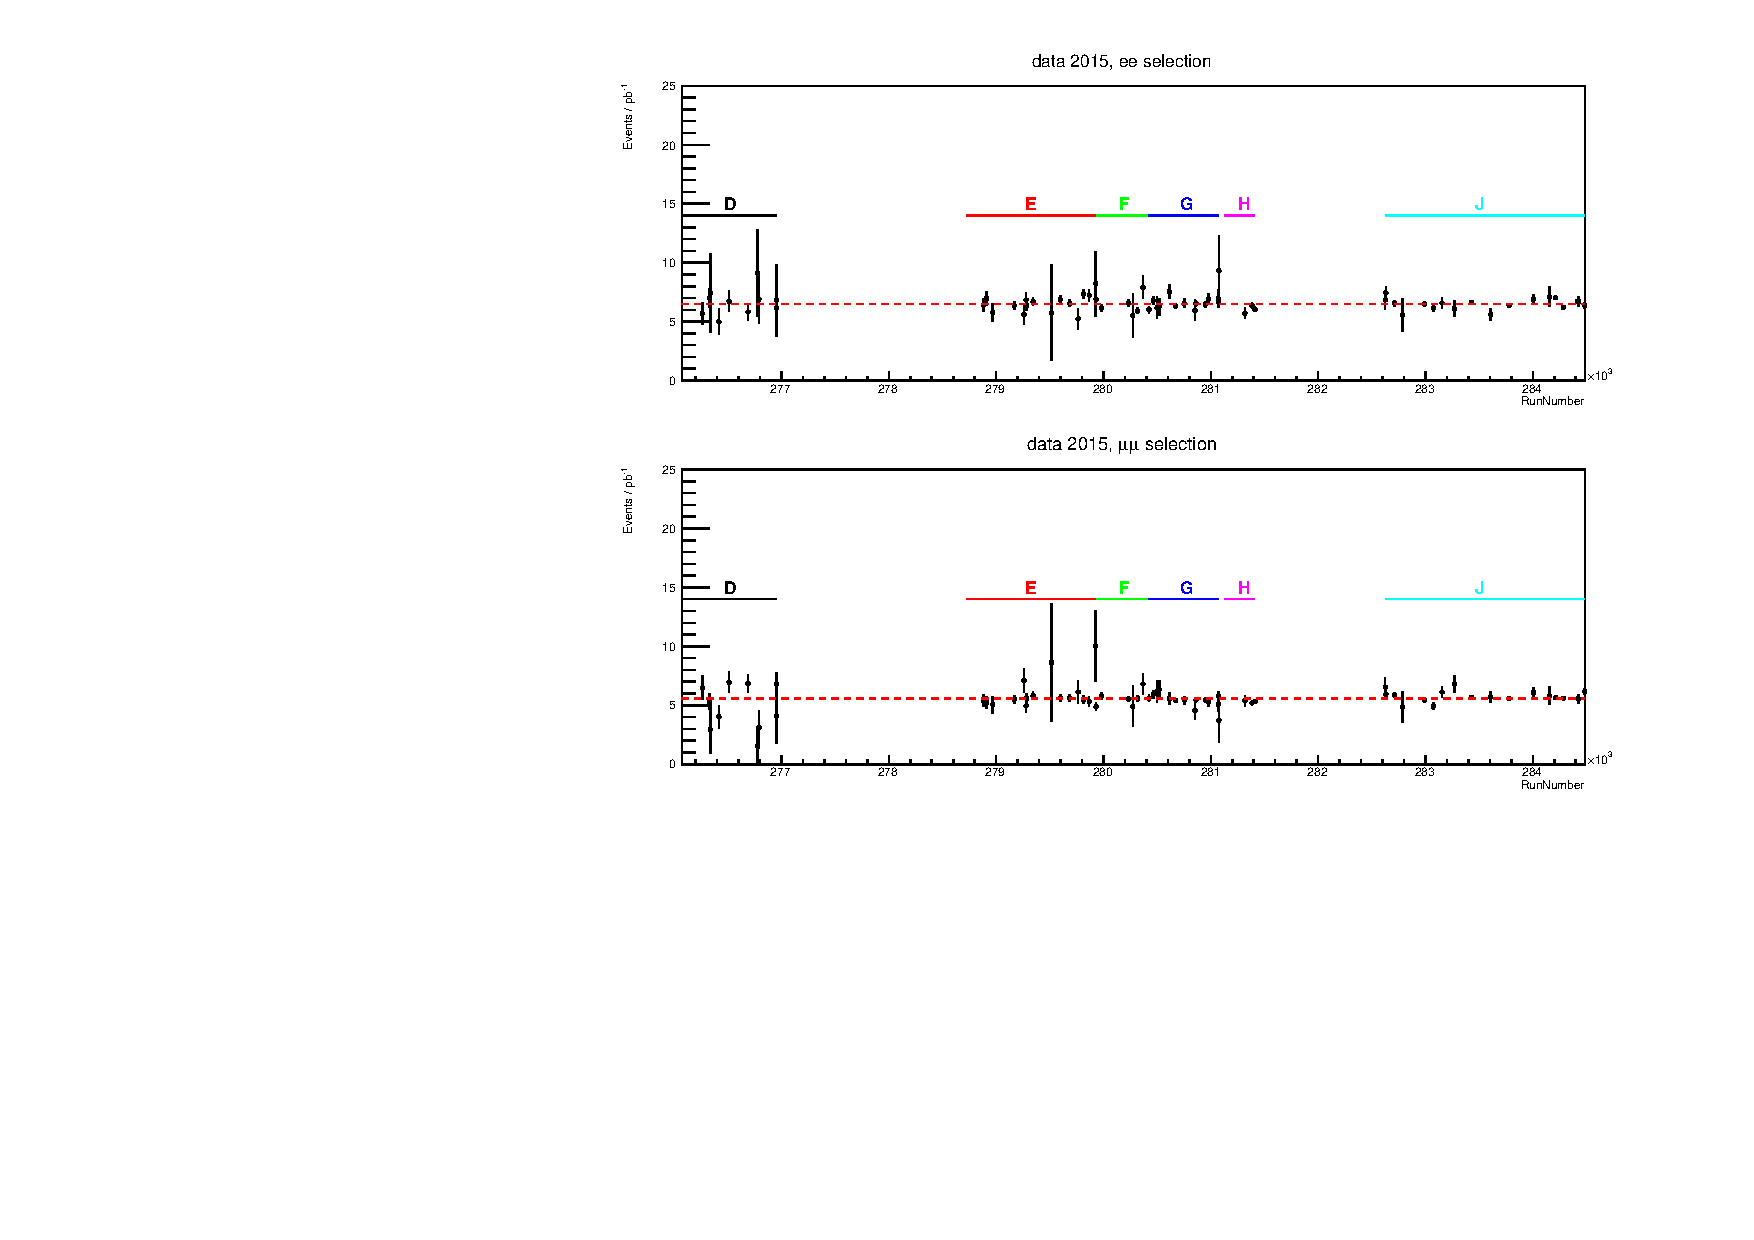
\includegraphics[width=\textwidth]{figures/analysis/datamc/Yields/compare_data_yields2015.pdf}
\caption{Data yields for the 2015 run period for the inclusive $ee$ (above) and $\mu\mu$ (below) selections. Each letter on the legend correspond to the different data taking periods within a year~\cite{Aad:2019fac}.}
\label{fig:yields2015}
\end{figure}

\begin{figure}[ht]
\centering
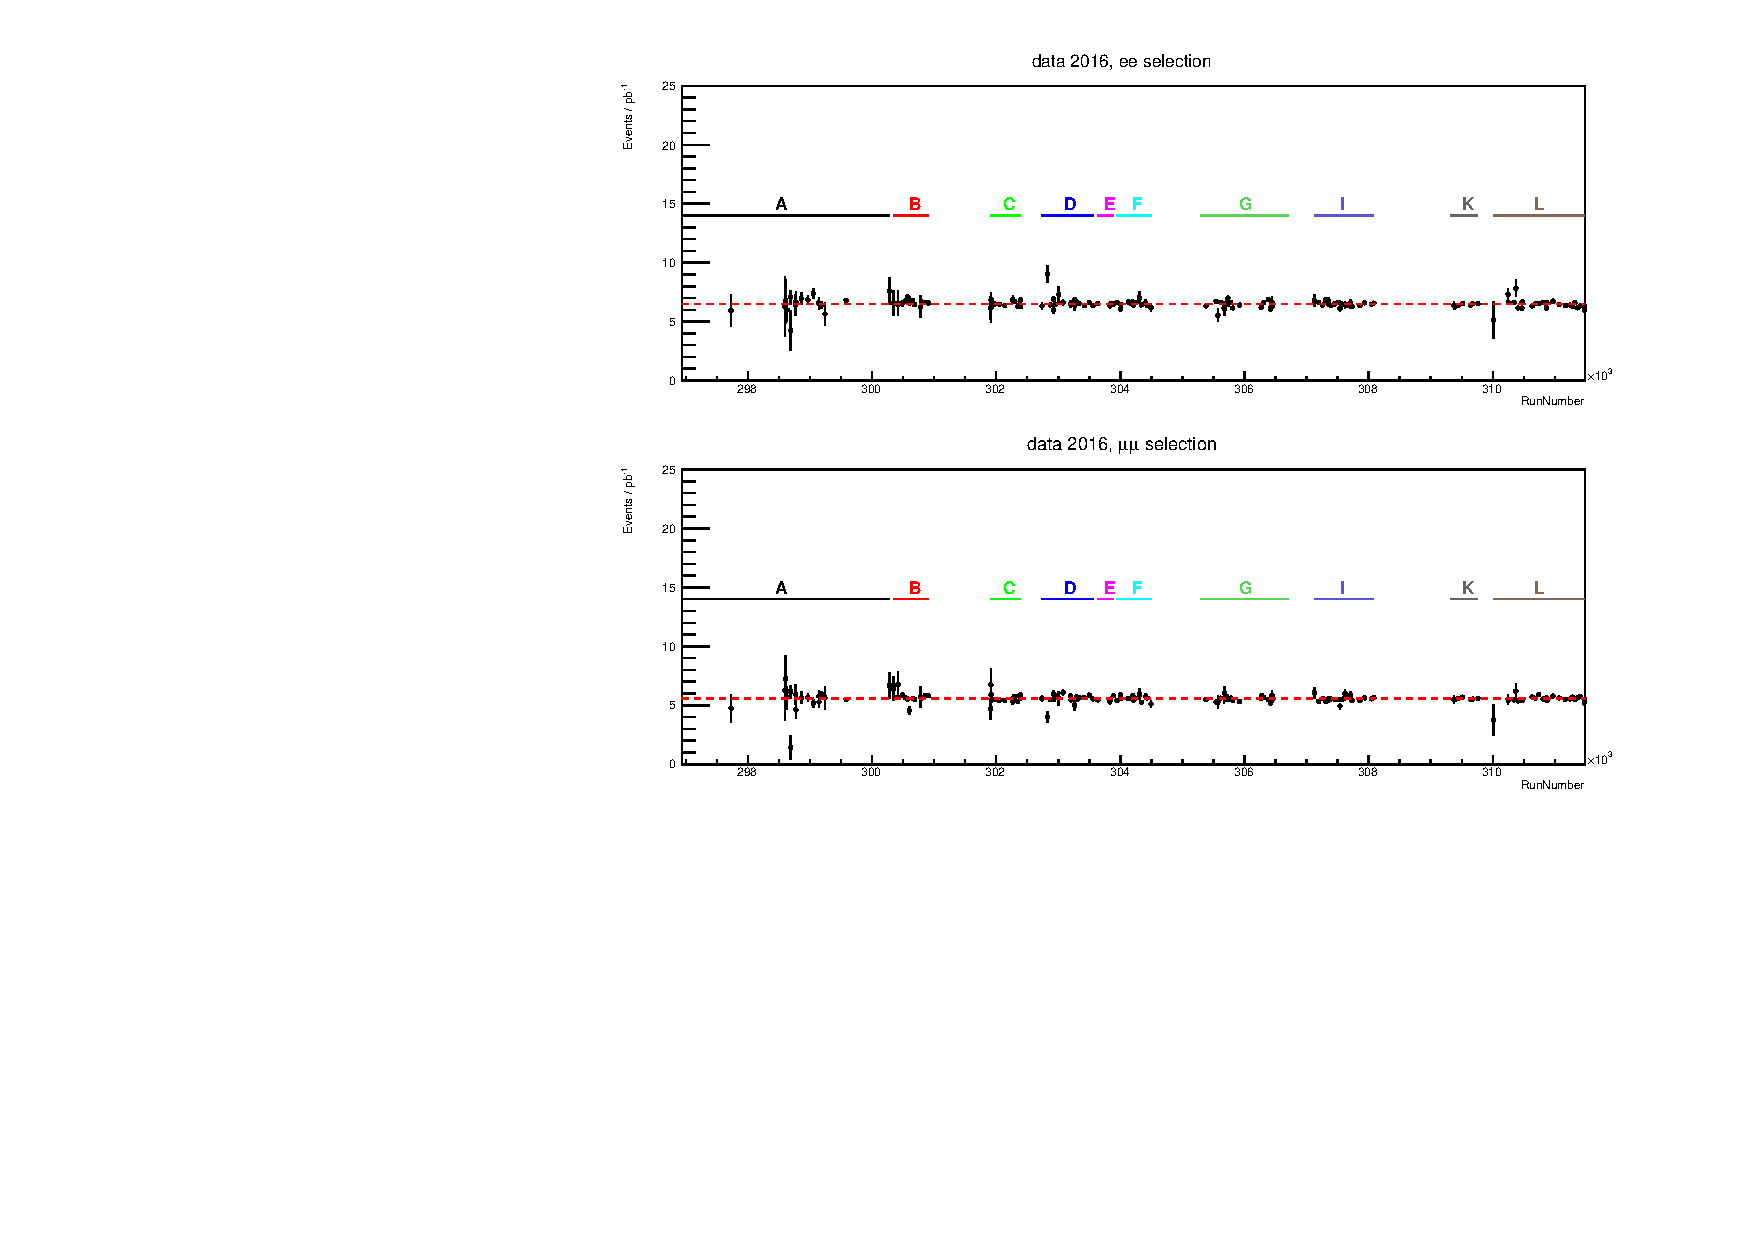
\includegraphics[width=\textwidth]{figures/analysis/datamc/Yields/compare_data_yields2016.pdf}
\caption{Data yields for the 2016 run period for the inclusive $ee$ (above) and $\mu\mu$ (below) selections. Each letter on the legend correspond to the different data taking periods within a year~\cite{Aad:2019fac}.}
\label{fig:yields2016}
\end{figure}

\begin{figure}[ht]
\centering
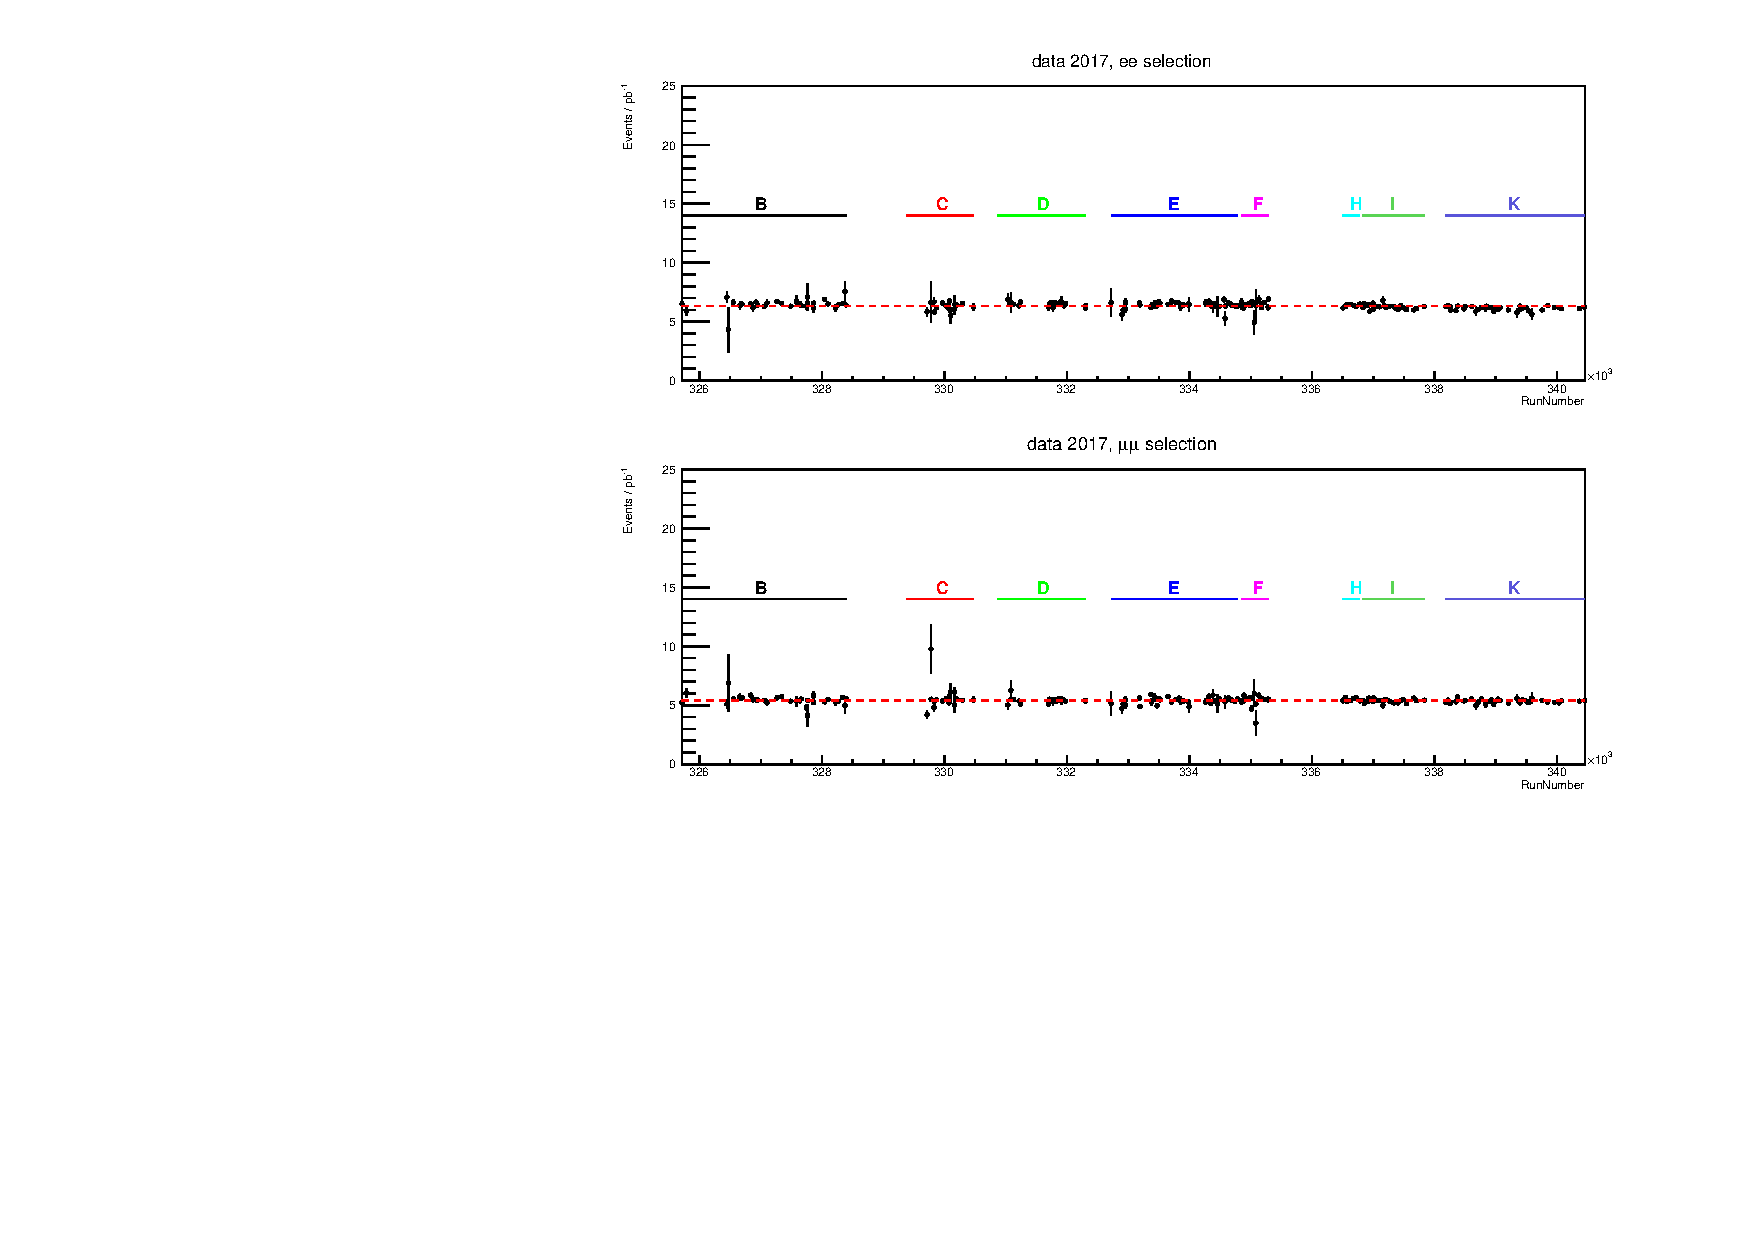
\includegraphics[width=\textwidth]{figures/analysis/datamc/Yields/compare_data_yields2017.pdf}
\caption{Data yields for the 2017 run period for the inclusive $ee$ (above) and $\mu\mu$ (below) selections. Each letter on the legend correspond to the different data taking periods within a year~\cite{Aad:2019fac}.}
\label{fig:yields2017}
\end{figure}

\begin{figure}[ht]
\centering
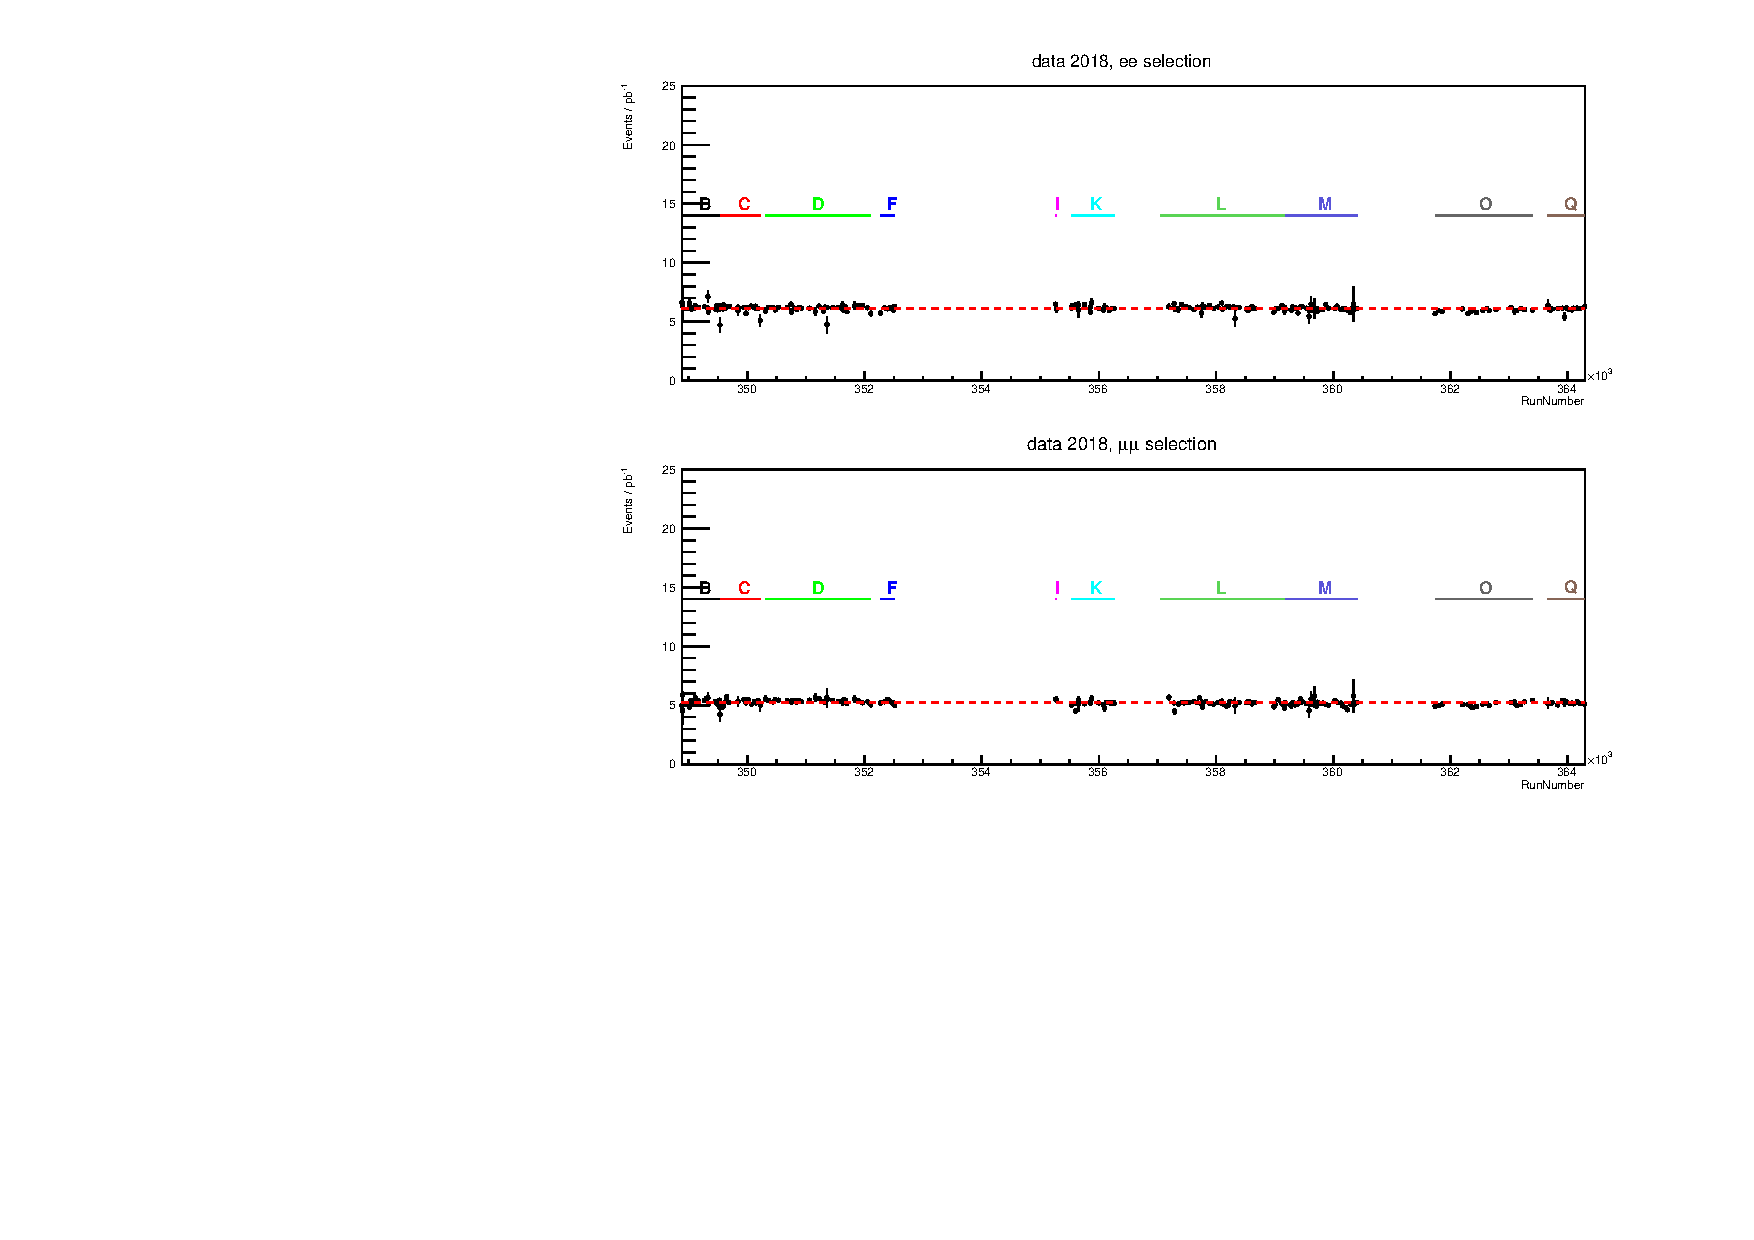
\includegraphics[width=\textwidth]{figures/analysis/datamc/Yields/compare_data_yields2018.pdf}
\caption{Data yields for the 2018 run period for the inclusive $ee$ (above) and $\mu\mu$ (below) selections Each letter on the legend correspond to the different data taking periods within a year~\cite{Aad:2019fac}.}
\label{fig:yields2018}
\end{figure}

\clearpage

\section{Monte Carlo samples}
While the analysis is carried out in a data driven way, simulated samples for the background and signal are used to determine the appropriate functional form to fit the data, study background compositions, estimate uncertainties and evaluate signal. This section outlines the MC samples used for the background and signal samples.

While generators are available to produce events using higher order matrix elements are now available, it is often required to enhance the description of the process beyond the order of the generator used. Higher order QCD and EW corrections can modify the shape of the invariant mass distributions. Mass-dependent \emph{K}-factors can be derived taking the ratio of the higher order differential cross-section calculation over the available sample, e.g. next-to-next-to-leading order(NNLO) over the next-to-leading order (NLO). The \emph{K}-factors can then be applied to the invariant mass distribution on an event by event basis to produce higher order samples. 

\subsection{Background samples}
The main backgrounds in decreasing order of importance are Drell-Yan (DY), top-quark ($t\bar{t}$), single-top-quark and diboson production. For the electron channel is it prohibitive to produce MC with enough events to accurately represent the expected QCD multijet distribution, due to the very small probabilities of jets faking electrons which pass the analysis selection. Therefore, the QCD and W+Jets processes in the dielectron channel are estimated with a data driven method~\cite{EXOT-2016-05}. For the muon channel the multijet background was studied and found to be negligible~\cite{EXOT-2016-05}, therefore, the contribution is neglected. 

The SM Drell-Yan process is modelled using the NLO \POWHEGBOX~\cite{Alioli:2010xd,Frixione:2007vw} event generator

\subsection{Signal samples}
